\chapter{Поиск предельного цикла}

Рассмотрим исследуемую систему (уравнение \ref{lab:eq:1},
$\nu$ - параметр системы). Она описывается
уравнением от одной фазовой переменной $x$. Уравнение дифференциальное, второго
порядка и, в силу слагаемого $3\dot{x}^3$, нелинейное. Решение такого уравнения
аналитическими методами является довольно сложной задачей, поэтому нашим
методом исследования будет построение численных экспериментов, описывающих
данную систему при определенном параметре $\nu$.

\begin{equation}\label{lab:eq:1}
  \ddot{x} + 3 \dot{x}^3 - \nu\dot{x} + x = 0
\end{equation}

Однако, в таком виде уравнение \ref{lab:eq:1} не является удобным для
моделирования. Поэтому приведем его к канонической форме от двух переменных, с
помощью замены \ref{lab:eq:2}, получив уравнение от двух фазовых переменных
$y_1$ и $y_2$ (Система уравнений \ref{lab:eq:3}). В дальнейшем, мы будем
пользоваться описанием нашей системы именно в таком виде.

\begin{equation}\label{lab:eq:2}
  \begin{cases}
    &y_1 = x \\
    &y_2 = \dot{x}
  \end{cases}
\end{equation}

\begin{equation}\label{lab:eq:3}
  \begin{cases}
    &\dot{y_1} = y_2 \\
    &\dot{y_2} = -3y_2^3\ + \nu y_2 - y_1
  \end{cases}
\end{equation}

Преобразовав систему к удобному для нас виду, перейдем к первой части работы --
нахождения такого параметра $\nu$, при котором наблюдается предельный цикл.

Для начала, дадим определение искомому объекту.

\begin{definition}\label{lab:def:cycle}
  Предельным циклом будем называть замкнутую изолированную траекторию
  в фазовом пространстве, подразумевая замкнутость в смысле периодичности
  поведения системы.
\end{definition}

Таким образом, нам нужно построить фазовый портрет нашей системы, на котором
нужно будет обнаружить искомую замкнутую линию. Для этого, зная зависимость
значения производных от их координат, можно с помощью функции
\textit{streamplot}\cite{streamplot} построить фазовый портрет (Программа
\ref{lab1:prog:1}, в качестве параметра для начала возьмем $\nu = 1$).

\begin{program}
  \caption{Построение фазового портрета}
  \label{lab1:prog:1}
  \begin{verbatim}
# Подключение используемых библиотек
# В дальнейшем является постоянным и опускается в листингах
# Полный исходный код программы можно найти в приложении
import matplotlib.pyplot as plt
import numpy as np

# Параметр системы
nu = 1

# создание сетки 100х100 точек в области [-3;3]x[-3;3]
Y, X = np.mgrid[-3:3:100j, -3:3:100j]

# вычисление фазовых векторов на сетке
Y1 = Y
Y2 = -3 * Y ** 3 + nu * Y - X

# построение фазового портрета
fig0, ax0 = plt.subplots()
plt.streamplot(X, Y, Y1, Y2)

# показать построенные графики (опускается в дальнейшем)
plt.show()
  \end{verbatim}
\end{program}
\clearpage


\begin{figure}[thp]
  \centering
  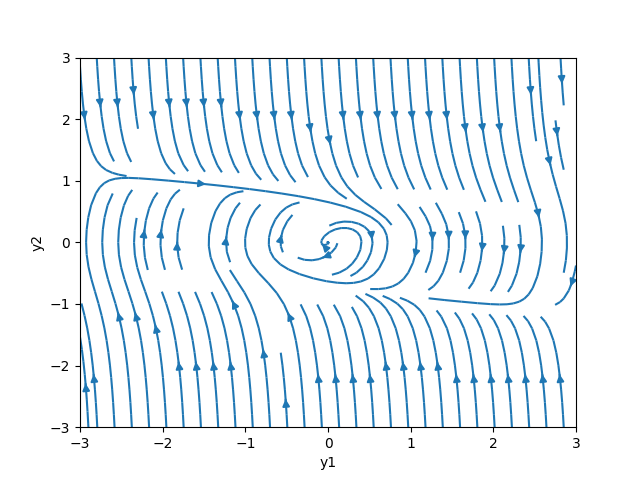
\includegraphics[width=\textwidth]{figures/1_streamplot}
  \caption{Поиск предельного цикла построением фазового портрета}
  \label{lab1:streamplot}
\end{figure}

На графике \ref{lab1:streamplot} изображен результат работы нашей программы.
В данном случае значение параметра оказалось оптимальным: можно видеть, как
изоклины сходятся к наклоненному прямоугольнику в центре графика.

Теперь, чтобы убедится наверняка, что траектории сходятся вокруг этого цикла
и там нет разрывов, построим две линии методом Эйлера снаружи и внутри наблюдаемого
цикла (Программа \ref{lab1:prog:2}).

\begin{program}
  \caption{Использование метода Эйлера для проверки предельного цикла}
  \label{lab1:prog:2}
  \begin{verbatim}
# функция построение кривой методом Эйлера
def line(y1_0, y2_0):
    y1 = [y1_0]
    y2 = [y2_0]
    h = 0.01 # длина шага
    for i in range(2000): # 200o - количество итераций
        y1.append(y1[i] + h*(y2[i]))
        y2.append(y2[i] + h*(-3*y2[i] ** 3 + nu*y2[i] - y1[i]))
    # отображение кривой на графике
    ax0.plot(y1, y2)

# построение двух кривых, начинающихся внутри и
# вне предполагаемого предельного цикла
line(0.1, 0.1)
line(2, 2)
  \end{verbatim}
\end{program}

\clearpage

\begin{figure}[thp]
  \centering
  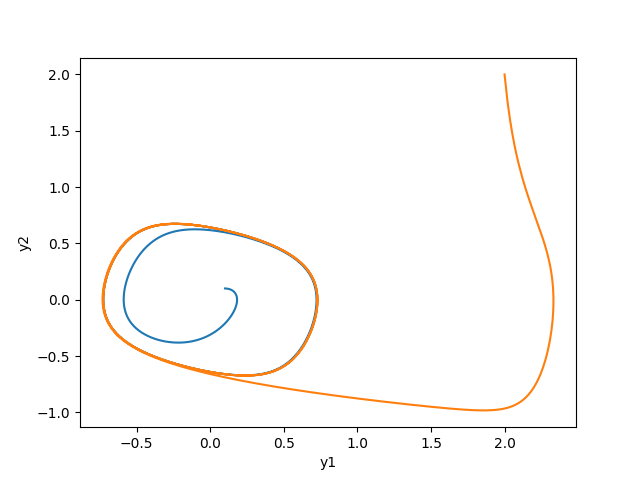
\includegraphics[width=\textwidth]{figures/1_cycle}
  \caption{Обнаружение аттрактора методом Эйлера}
  \label{lab1:cycle}
\end{figure}

На рисунке \ref{lab1:cycle} мы можем видеть две линии, начинающиеся из точек
$(0.1, 0.1)$ и $(2, 2)$. Эти линии сходятся сближаются к искомому предельному
циклу системы.
